% !TeX root = ../thesis_main.tex


\section{Solution Concept of DevContainers}\label{sec::solution_concept}
This section proposes the usage of Development Containers (DevContainers) as a solution to the problems of local development environments described in Section \ref{sec::problem}. The concept is oriented according to the \ac{PaaS} principles known in the cloud. Developers should only have to deal with the application. The runtime environment and network configuration are managed by the DevContainer. They combine the application runtime and its configuration into an isolated environment by using the lightweight virtualization approach of containers. One difference between DevContainers and the \ac{PaaS} principle is that DevContainers do not provide own hardware neither its management. \newline
The details of such a DevContainer concept are described below. This is followed by a delimitation of when its application scenarios make sense and when they do not. Finally, the advantages and limitations of this solution are outlined.

    \subsection{Description of a Conceptual Environment}
    The idea of DevContainers is to bundle the application code, its runtime and configuration into an isolated system. Only the minimal necessary scope for accessing the application is made available on the host system, all other resources remain isolated. According to the design of \ac{VM}s and containers, they can be started and stopped at will without the having the risk of contained applications causing permanent changes on the host system. When the container is started, all port, path and secret configurations are already set. Developers are not required to do any further manual configuration and additional steps. Different branches and versions of the applications all have their own container which are completely independent of the local settings. Auxiliary applications and interdependent services can all be started simultaneously and in the correct order. The DevContainer environment builds upon the Linux kernel and is completely independent of the host \ac{OS} and thus much closer to the production environment, potentially decreasing system specific errors. Even in case something goes wrong and the environment ends up in an undefined state, the principles from the server world can be applied. The DevContainer can simply be discarded and recreated from a well-defined template within seconds. Which even can enable environments that are 100\% reproducible.\newline
    Such a setup allows developers to choose any host \acl{OS} because all the application code is in a virtualized environment. It increases the initial setup time and prevents configuration drift because all configuration settings are following the \ac{IaC} principle and are stored as code. This way, new runtimes or dependencies can be tested without having to risk corrupting the local environment. Through automatic orchestration, integration tests become easier and can be performed earlier, shortening the time until an error is detected. Dependencies and common software like debugger are already present in the container, so they do not need to be installed separately. DevContainers promise to solve the problems described in Section \ref{sec::problem} and allow developers to focus on programming rather than configuring and maintaining their working environment.\newline
    Despite these potential advantages, DevContainers are not the miracle solution to all problems in software development. They have their limits and their area of application wich they are suitable for.

    \subsection{Pre-requirements for DevContainers}
    Before the use of DevContainers one has to verify hat these are the right approach for the encountered problems and that all necessary requirements are fulfilled.\newline
    DevContainers are based on virtualization technology, and one of their goals is to achieve the greatest possible similarity between the development and production environments. In order to take full advantage of this possibility, the production environment must already be designed for the use of virtualization with containers. As can be seen in Section \ref{ssec::toolsused}, the majority of virtualization solutions are based on Linux, which is also the most widely used system in the server domain. Applications that require Windows can also use Windows-based containers, but these may require additional licenses and configuration, accordingly they will not be discussed further in this paper. The application to be developed must be suitable for use in a container. Containers do not offer direct support of graphical output by default. Functions are exposed to the outside world via the usage of sockets or mounted devices. Experience in the area of virtualization and a functioning \ac{CI}/\ac{CD} pipeline for the rapid delivery of new application versions is therefore also recommended.\newline
    Although DevContainers reduce the configuration effort for each developer, the architecture and settings files for the use of DevContainers must be created once and then be maintained. As Section \ref{sssec::virtual} already shows, with any kind of virtualization, regardless of whether it is VMs or containers, there is a performance overhead. If, as in a typical microservice architecture, several applications are run at the same time, this overhead adds up and places an additional load on the developer's system. Modern hardware with sufficient memory and computing capacity is therefore necessary for the use of DevContainers. The amount of additional load depends on the technology stack used.

    \subsection{Creating a DevContainer setup}\label{ssec::toolsused}
    Section \ref{ssec::getting_devops} already presented concrete programs for providing the virtualization concept and automating certain processes with \ac{CI}. These form the basis for the provision of DevContainers. This must now be made available to developers in actual concepts and, in doing so, solve further problems described in Section \ref{sec::problem} as good as possible. Developers need to be able to initialize a DevContainer based environment quickly and must be offered a way to interact with the DevContainer, especially the application within, without significant impacting on their workflow. Therefore, tools and concepts that make this possible are presented below.

        \subsubsection{Defining the Application Runtime}
        The entire application runtime environment is virtualized using Docker. However, the basics of this runtime environment must be defined beforehand. In the case of Docker, this is done with Dockerfiles. These provide the build instructions for the Docker-images that are needed for a container in order to start. \ac{CI} platforms typically execute the building process of images automatically \cite{docker2020}.\newline
        % !TeX root = ../thesis_main.tex

\begin{lstlisting}[language=docker, frame=single, caption={Python DevContainer Dockerfile},label=code::docker_dev_example]
FROM debian:buster
RUN apt-get update && apt-get install -y \
    git python3 python3-pip make vim emacs && \
    pip3 install pandas numpy matpltlib pep8

Copy . /app #Optional
\end{lstlisting}

        Listing \ref{code::docker_dev_example} shows such a Dockerfile for a Python application. The Linux distribution Debian is chosen as the starting point for the image, followed by installation of all required dependencies and programs needed. There are two possibilities for implementing a DevContainer concept, when it comes to the source code. Optionally the program code can be copied into the image so that the image already contains all program components. The resulting fully self-contained image is the typical method in production operation. The disadvantage of this approach is that the program code can only be accessed within the container and is not present on the host system. While this is desirable in production, due to security and strict isolation, it results in additional development overhead. Developers can only use applications within the container to edit the code and the \ac{CI} system must create new images for every change. Prematurely discarded containers can lead to the loss of changes that have not yet been published to the remote source code repository \cite{dockerdocs}.\newline
        Alternatively, copying the program code can be omitted and only the well-defined runtime environment is provided in the image. The program code on the host system is then mapped into the container via a bind-mount at the start of the container. So the program code can be edited and used by any editor on the host. In the case of a discarded container, the changes made are still available on the host. Furthermore, a new image only needs to be created when something changes in the Dockerfile or dependencies, which saves a lot of computational effort in the \ac{CI} system. After the build process all images are than made available on a private or public image registry in oder to be accessible. In the working directory of the application the following commands are executed by the \ac{CI} system in order to create, name and upload the image to a registry:
        \begin{lstlisting}[language=bash, frame=none, numbers=none, backgroundcolor=\color{codebg}]
docker build -t my-python-app .
docker push my-python-app
        \end{lstlisting}
        \vspace{-1cm}

        \subsubsection{Orchestrating the Application Containers}
        In order for the Python application above to work, it needs a database. Instead of each developer having to install and set up a database on their own, which may then shared between different projects, this can be done in isolation and automatically for each project thanks to virtualization and composition of programs. Applications in an \ac{MSA} have even more services on which they depend on. Arranging all these programs into one greater service is called orchestration. Well-known applications for container based orchestration are \wordhighlight{Docker-Compose} and \wordhighlight{Kubernetes}. Since Kubernetes, does not ship with Docker by default, is quiet complex and production oriented, Docker-Compose is suggested for local orchestration.\newline
        Docker-Compose requires a configuration file, declared in the \acs{YAML} format, which contains all necessary information for orchestrating multiple applications. Each application is defined as a service with a unique name when using Docker-Compose. The \code{docker-compose.yml} file in Listing \ref{code::compose_example} defines the services \code{app} and \code{db}. Each service has an image which is the initial state for each container. With Docker containers, it is common to use environment variables to influence and configure the application within the container. The initial credentials for the database service are set via environment variables and the python app uses them to set the connection information to the database server. It should be noted that the database host can be simply the service name of the database server instead of an IP address. Within the Docker managed network, the integrated DNS server automatically resolves the service names to the IP address of the \ac{DB} server. This virtual network allows the containers to communicate with each other, but in order for the functionality to be available on the host, the network ports used must be explicitly exposed to the host. The Python application uses the alternative \acs{HTTP} port \code{8080} and the database server uses the standard MySQL port. When starting the containers, the corresponding ports are allocated on the host system and local programs can access the defined services using \code{localhost} and the corresponding network port \cite{dockerdocs}.\newline
        If the program code is not already copied into the image it must be mapped into the container using bind mount point. Line 11 in Listing \ref{code::compose_example} binds the local \code{app-src} directory from the host into the container at the location \code{/workspace}. The database service, on the other hand, uses a volume mount in which docker manages the allocated memory itself and persistently. The configuration is completed with an entry-point for the python app that will be executed when the container is started.\newline
        % !TeX root = ../thesis_main.tex

\begin{lstlisting}[language=docker-compose-2,caption={Exemplary Python Project \code{docker-compose.yml}},breaklines=true,label={code::compose_example}]
services:
  app:
    image: my-python-app
    entrypoint: python3 app.py
      - DB_HOST=db
      - DB_PW=yes
      - DB_USER=root
    ports:
      - 8080:8080
    volumes:
      ./app-src:/workspace

  db:
    image: mysql
    environment:
      - MYSQL_ROOT_PASSWORD=yes
    ports:
      - 3306:3306
    volumes:
      - sql_data:/var/lib/mysql
volumes:
  sql_data:
\end{lstlisting}

        Docker-Compose ensures interdependent services are started in the correct order, all persistent volumes are created, and all containers can communicate within their network \cite{docker2020}, \cite{dockerdocs}. Since the all necessary configurations are stored in an ordinary text-file, the \ac{IaC} principle can be applied here. The state all changes of the \code{docker-compose.yml} file are tracked in \ac{VCS}. Accordingly, even development work requiring changes to the runtime can take place in a separate branch without affecting the work of other developers.\newline
        Starting all services specified in the \code{docker-compose.yml} file is done with the console command \code{docker-compose up}. If the docker images used are not already present on the host, they are automatically downloaded from available image-registries. When all services are started, Docker-Compose attaches itself to all running containers and outputs all program output of each container color-coded to the console.\newline
        % \begin{lstlisting}[language=bash, frame=none, numbers=none, backgroundcolor=\color{codebg}]
        %     docker-compose up [app db]
        % \end{lstlisting}
        Through this concept, developers have isolated program environments that can be created quickly, easily and producible. Projects running in parallel no longer have to share a database-servers and different runtime environments, interpreters and compilers can be tested independently. In case a fast cache-server is needed, another service can be created quickly in order to provide a \wordhighlight{Redis} or \wordhighlight{Memcached} server without the need of installing it to the host. Individual, manual and diverging configurations for each developer are eliminated. New environments that are similar to the production environment can be created quickly, independent of the host operating system. Even in a microservice architecture, developers have the opportunity to test the interaction of multiple applications before committing changes to the \ac{VCS}. In this way, possible errors are already detected before CI integration tests, which means that they can be corrected more quickly. These characteristics promise to solve the problems described in Section \ref{sec::problem} regarding heterogeneity, lack of testing facilities, and the tedious configuration of the setup. In order for this concept to be adopted by developers, there must be an equivalently effective way for developers to interact with their applications within the DevContainer.

        \subsubsection{Interacting with DevContainers}
        The primary way developers interact with their code and the application is through their editor. Their variability and the number of different editors is great. Well known general purpose editors are Visual Studio, XCode, Atom, Sublime, Eclipse, Emacs and VIM. There is usually a distinction between simple text editors and \acl{IDE}. While text editors are quite simple and only provide basic functionalities like syntax highlighting, \ac{IDE}s are much more comprehensive with powerful IntelliSense suggestions, built-in project management, \ac{VCS}, debugger, graphical visualization and build-tools. The choice of the editor is a personal decision for most developers, and they are customized according to their preferences. For this reason, the proposed solution does not require a specific editor for DevContainers, but gives a recommendation that will be used as a reference for the rest of the work.\newline
        \ac{VSCode} is a free platform independent editor with extensive extendibility which is used by over 70\% of all developers accordingly to StackOverflow~\cite{stackoverflow2021}. One of its key beneficial features for virtualized workloads is its Remote Development functionally. This, officially provided, extension enables the intuitive comfort of a graphical \ac{UI} while running the code, the application and auxiliary processes like a debugger on another, remote machine. Figure \ref{fig::vscodecontainer} shows how the \ac{VSCode} frontend connects to a remote machine or container and installs a server instance of the editor. The server side instance manages access to the remote file system and the execution of processes while communicating with the local \ac{VSCode} frontend instance for comfortable access to these functions. This type of remote development works for \ac{SSH} connections, the \ac{WSL}, and on Docker containers. \ac{WSL} is a built-in Windows feature to provide a Linux environment on Windows hosts without the need of a separated \ac{VM}. The implementation of Docker for Windows is build upon this functionality \cite{vscodedevcontainer}. In the further course, only the remote functionality for containers will be considered.
        \begin{figure}[]
            \centering
            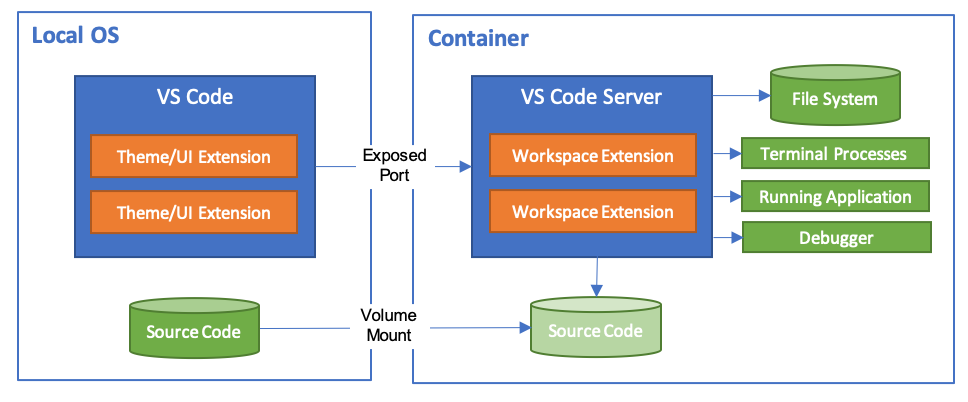
\includegraphics[width=.95\textwidth]{architecture-containers.png}
            \caption{Architecture of \ac{VSCode} Development Container Setup \\\textit{Source:~\cite{vscodedevcontainer}}}\label{fig::vscodecontainer}
        \end{figure}
        In order for container services to be accessed, the appropriate ports are exposed via Docker-Compose, \ac{VSCode} provides a similar feature through the remote extension. Remote processes on one host are automatically made available locally through port forwarding. Since this functionality is not available for multiple containers simultaneously, this feature is only useful for a service which is currently being worked on or services with dynamically changing network ports. However, this feature can be used to quickly make a short-lived process available on the host without having to modify the configuration in the \code{docker-compose.yml} file. This allows the usage of local testing or exploration tools on any remote services.\newline
        In order for \ac{VSCode} to connect to or start a DevContainer, a configuration file is required. This is provided by a \code{devcontainer.json} file. For each service being developed, the path to the \code{docker-compose.yml} file is specified and to which service \ac{VSCode} should connect to. Listing \ref{code::devcontainer_json} shows such a configuration file. It also specifies which directory the \ac{VSCode} server should open, which extensions have be installed and what happens when the container starts or stops. If this file is present, \ac{VSCode} automatically offers to reload the local project using the DevContainer. All services are started automatically, directories are mounted, and the network ports are allocated accordingly. Thus, the development work is nearly identical to a local setup \cite{vscodedevcontainer}.\newline
        % !TeX root = ../thesis_main.tex

\begin{lstlisting}[language=json,caption={\ac{VSCode}s Remote Container \code{devcontainer.json} Configuration File},breaklines=true,label={code::devcontainer_json}]
{
  "name": "MY-PYTHON-APP",

  // Path to the docker-compose.yml file.
  "dockerComposeFile": ["../../docker-compose.yml"],

  // The service property for the container that VSCode uses.
  "service": "app",

  // The project folder to be opened by VSCode when connected.
  // Keep your containers running after VS Code shuts down.
  "workspaceFolder": "/workspace",
  "shutdownAction": "none",

  // Extensions to be installed when the container is created.
  "extensions": [
      "ms-python.python",
      "ms-python.vscode-pylance"
  ],

  // Runs this command after the container is created
  "postCreateCommand": "/workspace/.devcontainer/kill_app.sh"
}


\end{lstlisting}

        All these functions can be archived without \ac{VSCode} by using remote filesystem mounts, (\ac{SSH}) port-forwarding or terminal based editors. Even without VSCode, any file changes made by any editor in the container will take effect, since the source code directories are bind-mounted. Nerveless, it cannot be ruled out that when using editors other than \ac{VSCode}, adjustments to the \code{docker-compose.yml} file may are necessary compared to the setup described in Section \ref{ssec::imp_approach}.

        \subsubsection{Variations and Additional Supporting Tools}
        In addition to the tools mentioned above and in Section \ref{ssec::getting_devops}, other auxiliary programs can be used. To simplify certain workflows and automate recurring tasks scripts will be used. The \wordhighlight{Bash} scripting language can be used natively on Linux and macOS, the installation of Git for Windows also brings Bash support to Windows. Accordingly, one uniform scripting language can be used to perform platform-independent operations and to simplify complex instructions. In order that developers do not have to wait for the creation of the DevContainer images, these should be built automatically by a Ci and made available in a private container registry. Accordingly, uniform and up-to-date images are always available to all developers. \newline
        It is also possible to use other management tools via Docker. Database management tools such as \wordhighlight{PHP-MyAdmin} can simplify administration by adding further services. The same applies to the management of containers via \wordhighlight{Portainer}. Although Docker-Compose offers a color-coded log output, even this can become overwhelming if there are too many logs. Since the Docker stack is used anyway, enterprise log aggregators and analysis tools like \wordhighlight{Grafana} or \wordhighlight{Elastic-Search} can be used to get a persistent and searchable log dashboard.

    \subsection{Security Aspects of this Concept}\label{ssec::sec}
    The presented solution is oriented to the development process and not to productive operation. For this reason, common security practices for container operation are not implemented. The images contain extra programs that are not mandatory but convenient. The processes in the container run as super-user to avoid additional configuration effort and interruptions due to access errors. In the \code{docker-compose.yml} file, passwords are defined in plain text to allow consistent and easy setup across any number of systems. Functions and data within the containers are made available through exposed ports on the host. Accordingly, it must be ensured that the host is not accessible from the Internet. If certain services such as databases or log dashboards are shared between developers through a central server, it must be ensured that this server is only accessible within the company network in order to avoid the unintentional publication of confidential information. The same security measures must be applied as for a non-containerized local development environment.

    \subsection{Strengths, Weaknesses and Limits}\label{ssec::limits}
    The software and methods described in Section \ref{ssec::toolsused} are already standard practice in DevOps enabled teams. Accordingly, the entry barrier is small in compared to new and unknown tools. DevContainer allow for a homogenization of development and production environment. The application runtime is identical, accordingly \ac{OS} or runtime specific errors are prevented. Developers can use a ready to go development project setups without having to install and configure the application runtime themselves. Dependencies, keys, supporting tools like debuggers and configurations can already be shipped within the container to enable a quick initial setup. Instead of examining the environment for a long time in the event of an error it can quickly been torn down and recreated into a known good state. These are the key features that DevContainer promise to provide, in addition to solutions to the problems described in Section \ref{sec::problem}. They extend the existing toolset of agile and DevOps teams with another tool that allows developers to be more flexible and focus more on coding.\newline
    It should be noted that DevContainers are not a perfect solution to all problems in the software development stack. Like any other tool they come with their own set of quirks. Expertise for the use of Docker containers must be available, and the production architectural must be transformable to a local DevContainer-based configuration. This configuration must be kept up to date and be maintained. Developers may need to adapt to minor adjustments in their workflow. The \ac{CI}/\ac{CD} solution used must always be available and provide up-to-date container images. Every virtualization approach creates an additional overhead that cannot be ignored, especially when using multiple containers on Windows based systems. Details of the exact effects are given in Section \ref{sec::eval}.\newline
    As mentioned before, there are also projects for which the use of DevContainers is simply not suitable. Heavy monolithic applications are not in the sense of containers and therefore not suitable for DevContainers. Graphical applications can run in containers but require a graphical X-Server on the host and the resulting experience is not comparable to a native \ac{UX}. Similar limitations apply to applications that require a Windows stack. This can be implemented, but is no longer platform-independent, requires additional licenses and further adaptations. For embedded projects that require specific hardware, a virtualization approach is just not feasible and accordingly these are also not suitable for DevContainers.\newline
    To demonstrate a suitable use of DevContainers, the next section describes how to migrate from a traditional development environment to a DevContainer-based solution based on a real project.

\subsection{Alternative Solutions}\label{ssec::alternatives}
Besides the solution concept presented here, there are already alternative solutions on the market that promise to solve similar problems as in section \ref{sec::problem}. A selecting of these solutions is presented in the following. These alternative virtualization-based development environments can be roughly classified into two categories. Purely browser based and container based solutions. A comparison of these to the solution presented here will be described in Section \ref{sses::eval_compare}.
\myparagraph{Browser based Development Enviorments}
Browser based development solutions provide an editor that is entirely built upon of web technologies. Therbey they can run on every device with a modern web-browser. Their goal is to provide a quick functioning setup without any configuration.\newline
The products codesandbox.io and Stackblitz implement this approach. Both solutions offer a \ac{VSCode}-like editor in the browser and allow the development of NodeJS based JavaScript projects.
While codesandbox.io provides the server-side infrastructure und functionality themselves and developers are dependent on an Internet connection, Stackblitz can also be used without an Internet connection. Stackblitz is a \ac{PWA} which brings the nodeJS runtime into the browser by using Webassembly. While codesandbox.io does not provide any console at all and the management is completely done by the service provider, Stackblitz provides a minimal shell for installing, copying and launching files. However, since both solutions run within the browser, it is not possible to open any regular TCP/UDP ports due to the security regulations of browsers. Network connections are only made available via the http based WebSockets protocoll \cite{codesandbox}, \cite{stackblitz}.

\myparagraph{Container based Development Enviorments}
Similar to the solution presented in this paper, containers are used in which theoretically everything can be installed. Compared to browser-based solutions, container-based development environments offer broader functionality and are not restricted on one specific programming language. The best-known products that implement this are GitPod and GitHub's Codespaces, which was not released until 2021. The infrastructure for the containers is provided by the provider, but GitPod also offers a self-hosting option. There are no restrictions for users in the containers, additional software can be added as desired, and regular network ports can also be opened to the outside. Both solutions can be used in the browser as well as in a local \ac{VSCode} installation via the remote development extension.\newline
Both services are billed either on a monthly basis or on an hourly usage basis \cite{githubcodespace}, \cite{gitpod}.
